
\documentclass[main.tex]{subfiles}
\begin{document}

\chapter{Derivation of the Flow Coefficients}
\label{outflows:coefficients-derivation}

\begin{figure}
\centering
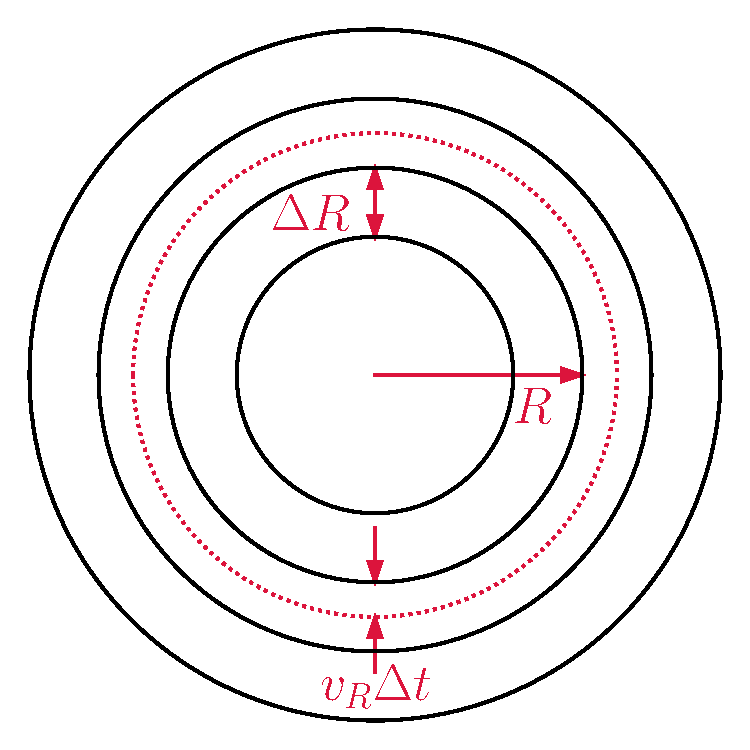
\includegraphics[scale = 0.5]{chapter7/schematic.pdf}
\caption{
A schematic of our derivation of the flow coefficients~$\mu_\flow$
and~$\gamma_\flow$.}
\label{outflows:fig:coefficients-schematic}
\end{figure}

\begin{itemize}

	\item The goal is to motivate a parameterization that includes the effect
	of radial gas flows in one-zone GCE models.
	Here we present the derivation of the coefficients~$\mu_\flow$ and
	$\gamma_\flow$ introduced in~\S~X.Y.Z.

	\item Consider a ring embedded in the Milky Way disk spanning the radial
	range~$R \rightarrow R + \Delta R$ which is described by a one-zone model.
	In the limit of a single, uniform inward flow velocity~$v_R$, all of the
	ISM material in the range~$R \rightarrow R + v_R \Delta t$ will be lost
	to the next ring inward in one differential timestep of size~$\Delta t$.
	Fig.~\ref{outflows:fig:coefficients-schematic} shows a schematic of this
	spatial configuration.
	The mass that migrates inward can then be expressed according to the
	area fraction~$a$ given by
	\begin{equation}\begin{split}
	a &\equiv \frac{
		\pi \left(R + v_R \Delta t\right)^2 - R^2
	}{
		\pi \left(R + \Delta R\right)^2 - R^2
	}
	\\
	&= \frac{
		2 R v_R \Delta t + v_R^2 \Delta t^2
	}{
		2 R \Delta R + \Delta R^2
	}.
	\label{outflows:eq:area-frac-def}
	\end{split}\end{equation}
	Simultaneously, material will be gained from the next ring out, spanning
	radii~$R + \Delta R \rightarrow R + 2\Delta R$.
	The net flow rate of some element~$x$ can then be expressed as the
	difference of these two source and sink terms:
	\begin{equation}\begin{split}
	\dot{M}_{x,\flow} &= \dot{M}_{x,\flow,\text{in}} -
	\dot{M}_{x,\flow,\text{out}}
	\\
	&= Z_x(R + \Delta R) M_g(R + \Delta R) \frac{a(R + \Delta R)}{\Delta t} -
	Z_x(R) M_g(R) \frac{a(R)}{\Delta t},
	\label{outflows:eq:flowin-minus-flowout}
	\end{split}\end{equation}
	where~$Z_x \equiv M_x / M_g$ is the mass-fraction of the element~$x$ in the
	ISM and~$M_g$ is the mass of the ISM gas itself.

	\item Regardless of the functional form of~$Z_x(R)$ and~$M_g(R)$, they can
	be expressed in terms of a Taylor series, along with~$a$:
	\begin{subequations}\begin{align}
	Z_x(R + \Delta R) &= Z_x(R) +
	\sum_{i = 1}^\infty \frac{\partial^i Z_x}{\partial R^i} \Delta R^i
	\\
	M_g(R + \Delta R) &= M_g(R) +
	\sum_{i = 1}^\infty \frac{\partial^i M_g}{\partial R^i} \Delta R^i
	\\
	a(R + \Delta R) &= a(R) +
	\sum_{i = 1}^\infty \frac{\partial^i a}{\partial R^i} \Delta a^i.
	\end{align}\end{subequations}
	Although it is straightforward to evaluate~$a(R + \Delta R)$ with the
	transformation~$R \rightarrow R + \Delta R$ in
	equation~\refp{outflows:eq:area-frac-def}, it is notationally convenient to
	this derivation to write it in terms of a Taylor expansion.
	Plugging these expressions into
	equation~\refp{outflows:eq:flowin-minus-flowout}:
	\begin{equation}\begin{split}
	\dot{M}_{x,\flow} &= Z_x(R) M_g(R)
	\frac{2 R v_R + v_R^2 \Delta t}{2 R \Delta R + \Delta R^2}
	\Bigg[
	\left(1 + \frac{1}{Z_x(R)}
	\sum_{i = 1}^\infty \frac{\partial^i Z_x}{\partial R^i} \Delta R^i\right)
	\\
	&\quad
	\left(1 + \frac{1}{M_g(R)}
	\sum_{i = 1}^\infty \frac{\partial^i M_g}{\partial R^i} \Delta R^i\right)
	\left(1 + \frac{1}{a(R)}
	\sum_{i = 1}^\infty \frac{\partial^i a}{\partial R^i} \Delta R^i\right)
	- 1\Bigg].
	\end{split}\end{equation}

	\item At this point, we take the limit of the above expression as
	$\Delta R$ and $\Delta t \rightarrow 0$ to parameterize the flow rate in a
	manner that is independent of these arbitrary choices of the ring width and
	the timestep size.
	For notational convenience, we let~$\Gamma$ denote the quantity in square
	brackets:
	The limit as~$\Delta t \rightarrow 0$ is trivial:
	\begin{equation}
	\lim_{\Delta t \rightarrow 0} \dot{M}_{x,\flow} = Z_x(R) M_g(R)
	\frac{2 R v_R}{2 R \Delta R + \Delta R^2} \Gamma,
	\end{equation}
	but the limit as~$\Delta R \rightarrow 0$ requires L'H\^opital's Rule since
	both~$2 R \Delta R + \Delta R^2$ and~$\Gamma \rightarrow 0$.
	Taking the derivative of~$\Gamma$ with respect to~$\Delta R$ to this end:
	\begin{subequations}\begin{align}
	\lim_{\Delta R \rightarrow 0} \dot{M}_{x,\flow} &=
	Z_x(R) M_g(R) \left( \frac{2 R v_R}{2R + 2 \Delta R} \right)
	\frac{\partial \Gamma}{\partial \Delta R}
	\\
	\begin{split}
	\frac{\partial \Gamma}{\partial \Delta R} &=
	\left(\frac{1}{Z_x} \sum_{i = 1}^\infty i
	\frac{\partial^i Z_x}{\partial R^i} \Delta R^{i - 1}\right)
	\left(1 + \frac{1}{M_g(R)}
	\sum_{i = 1}^\infty \frac{\partial^i M_g}{\partial R^i} \Delta R^i\right)
	\\
	&\quad
	\left(1 + \frac{1}{a(R)}
	\sum_{i = 1}^\infty \frac{\partial^i a}{\partial R^i} \Delta R^i\right) +
	\\
	&\quad
	\left(1 + \frac{1}{Z_x(R)}
	\sum_{i = 1}^\infty \frac{\partial^i Z_x}{\partial R^i} \Delta R^i\right)
	\left(\frac{1}{M_g} \sum_{i = 1}^\infty i
	\frac{\partial^i M_g}{\partial R^i} \Delta R^{i - 1}\right)
	\\
	&\quad
	\left(1 + \frac{1}{a(R)}
	\sum_{i = 1}^\infty \frac{\partial^i a}{\partial R^i} \Delta R^i\right) +
	\\
	&\quad
	\left(1 + \frac{1}{Z_x(R)}
	\sum_{i = 1}^\infty \frac{\partial^i Z_x}{\partial R^i} \Delta R^i\right)
	\left(1 + \frac{1}{M_g(R)}
	\sum_{i = 1}^\infty \frac{\partial^i M_g}{\partial R^i} \Delta R^i\right)
	\\
	&\quad
	\left(\frac{1}{a} \sum_{i = 1}^\infty i \frac{\partial^i a}{\partial R^i}
	\Delta R^{i - 1}\right).
	\end{split}
	\end{align}\end{subequations}
	Since we are taking the limit as~$\partial \Gamma / \partial \Delta R$
	approaches zero, despite the complicated nature of its expression, all but
	terms with~$\Delta R^{i - 1}$ with~$i = 1$ drop out entirely.
	This results in the following expression for~$\dot{M}_{x,\flow}$:
	\begin{equation}
	\dot{M}_{x,\flow} = Z_x(R) M_g(R) v_R \left(
	\frac{1}{Z_x} \frac{\partial Z_x}{\partial R} +
	\frac{1}{M_g} \frac{\partial M_g}{\partial R} +
	\frac{1}{a} \frac{\partial a}{\partial R}
	\right).
	\end{equation}

\end{itemize}

\end{document}

































